%%%%%%%%%%%%%%%%%%%%%%%%%%%%%%%%%%%%%%%%%
% Journal Article
% LaTeX Template
% Version 1.4 (15/5/16)
%
% This template has been downloaded from:
% http://www.LaTeXTemplates.com
%
% Original author:
% Frits Wenneker (http://www.howtotex.com) with extensive modifications by
% Vel (vel@LaTeXTemplates.com)
%
% License:
% CC BY-NC-SA 3.0 (http://creativecommons.org/licenses/by-nc-sa/3.0/)
%
%%%%%%%%%%%%%%%%%%%%%%%%%%%%%%%%%%%%%%%%%

%----------------------------------------------------------------------------------------
%	PACKAGES AND OTHER DOCUMENT CONFIGURATIONS
%----------------------------------------------------------------------------------------

\documentclass[twoside,twocolumn]{article}

\usepackage{blindtext} % Package to generate dummy text throughout this template 

\usepackage{hyperref}
\hypersetup{
    colorlinks=true,
    linkcolor=blue,
    filecolor=magenta,      
    urlcolor=cyan,
}

\usepackage[sc]{mathpazo} % Use the Palatino font
\usepackage[T1]{fontenc} % Use 8-bit encoding that has 256 glyphs
\linespread{1.05} % Line spacing - Palatino needs more space between lines
\usepackage{microtype} % Slightly tweak font spacing for aesthetics
\usepackage[utf8]{inputenc}

\usepackage[portuguese]{babel} % Language hyphenation and typographical rules

\usepackage[hmarginratio=1:1,top=32mm,columnsep=20pt]{geometry} % Document margins
\usepackage[hang, small,labelfont=bf,up,textfont=it,up]{caption} % Custom captions under/above floats in tables or figures
\usepackage{booktabs} % Horizontal rules in tables

\usepackage{lettrine} % The lettrine is the first enlarged letter at the beginning of the text
\usepackage{float}
\usepackage{enumitem} % Customized lists
\setlist[itemize]{noitemsep} % Make itemize lists more compact

\usepackage{abstract} % Allows abstract customization
\renewcommand{\abstractnamefont}{\normalfont\bfseries} % Set the "Abstract" text to bold
\renewcommand{\abstracttextfont}{\normalfont\small\itshape} % Set the abstract itself to small italic text
%\usepackage[shortlabels]{enumitem}
\usepackage{enumitem}
\usepackage{titlesec} % Allows customization of titles
\renewcommand\thesection{\Roman{section}} % Roman numerals for the sections
\renewcommand\thesubsection{\roman{subsection}} % roman numerals for subsections
\titleformat{\section}[block]{\large\scshape\centering}{\thesection.}{1em}{} % Change the look of the section titles
\titleformat{\subsection}[block]{\large}{\thesubsection.}{1em}{} % Change the look of the section titles

\usepackage{fancyhdr} % Headers and footers
\pagestyle{fancy} % All pages have headers and footers
\fancyhead{} % Blank out the default header
\fancyfoot{} % Blank out the default footer
\fancyhead[C]{MO443 $\bullet$ Junho 2019 $\bullet$ Relatório 04} % Custom header text
\fancyfoot[RO,LE]{\thepage} % Custom footer text

\usepackage{titling} % Customizing the title section

\usepackage{hyperref} % For hyperlinks in the PDF

\usepackage{graphicx}
\usepackage{subfigure}

\usepackage{mathtools}
\DeclarePairedDelimiter\floor{\lfloor}{\rfloor}
%----------------------------------------------------------------------------------------
%	TITLE SECTION
%----------------------------------------------------------------------------------------

\setlength{\droptitle}{-4\baselineskip} % Move the title up

\pretitle{\begin{center}\Huge\bfseries} % Article title formatting
\posttitle{\end{center}} % Article title closing formatting
\title{Relatório - Trabalho 04 \\ \Large MO443 - Introdução ao Processamento de Imagem Digital} %
%\subtitle{qsdqwdqwd} %Article title
\author{%
\textsc{Vinicius Teixeira de Melo - RA: 230223} \\[1ex] % Your name
\normalsize Universidade Estadual de Campinas \\ % Your institution
\normalsize \href{mailto:viniciusteixeira@liv.ic.unicamp.br}{viniciusteixeira@liv.ic.unicamp.br} % Your email address
%\and % Uncomment if 2 authors are required, duplicate these 4 lines if more
%\textsc{Jane Smith}\thanks{Corresponding author} \\[1ex] % Second author's name
%\normalsize University of Utah \\ % Second author's institution
%\normalsize \href{mailto:jane@smith.com}{jane@smith.com} % Second author's email address
}
\date{\today} % Leave empty to omit a date
\renewcommand{\maketitlehookd}{%
%\begin{abstract}
%\noindent \blindtext % Dummy abstract text - replace \blindtext with your abstract text
%\end{abstract}
}

%----------------------------------------------------------------------------------------

\begin{document}

% Print the title
\maketitle

%----------------------------------------------------------------------------------------
%	ARTICLE CONTENTS
%----------------------------------------------------------------------------------------

\section{Especificação do Problema}

O objetivo deste trabalho é aplicar técnicas de detecção de pontos de interesse para registrar um par de imagens e criar uma imagem panorâmica formado pela ligação entre as imagens após sua correspondência.

Os principais passos do processo de correspondência e geração da imagem panorâmica são:

\begin{enumerate}
	\item converter as imagens coloridas de entrada em imagens de níveis de cinza;
	\item encontrar pontos de interesse e descritores invariantes locais para o par de imagens;
	\item computar distâncias (similaridades) entre cada descritor das duas imagens;
	\item selecionar as melhores correspondências para cada descritor de imagem;
	\item executar a técnica \textit{RANSAC} (\textit{RANdom SAmple Consensus}) para estimar a matriz de homografia (\textit{cv2.findHomography}).
	\item aplicar uma projeção de perspectiva (\textit{cv2.warpPerspective}) para alinhar as imagens;
	\item unir as imagens alinhadas e criar a imagem panorâmica;
	\item desenhar retas entre pontos correspondentes no par de imagens.
\end{enumerate}

No passo (2), é necessário explorar e comparar diferentes detectores de pontos de interesse e descritores, tais como \textit{SIFT} (\textit{Scale Invariant Feature Transform}), \textit{SURF} (\textit{Speed Up Robust Feature}), \textit{BRIEF} (\textit{Robust Independent Elementary Features}) e \textit{ORB} (\textit{Oriented FAST, Rotated BRIEF}). No passo (4), uma correspondência será considerada se o limiar definido estiver acima de um valor especificado pelo usuário. No passo (5), o cálculo da matriz de homografia requer o uso de, no mínimo, 4 pontos de correspondência.

A fundamentação e resolução deste trabalho estão descritar nas seções seguintes.

%------------------------------------------------

\section{Entrada de Dados}

O código fonte criado para a execução de todas as tarefas está no notebook \textbf{Trabalho 04.ipynb}. O código foi criado para aceitar imagens coloridas ou em escala de cinza em diversos formatos, como exemplo: \textit{PNG} (\textit{Portable Network Graphics}), \textit{JPG} (\textit{Joint Photographic Group}), entre outros.

Para executar o notebook, basta iniciar o ambiente \textit{Jupyter Notebook}, abrir o notebook \textbf{Trabalho 04.ipynb} e executar as células em ordem. Todo o algoritmo foi implementado na linguagem Python na versão 3.6.

As imagens de entrada utilizadas nso testes dos algoritmos foram retiradas da página do prof. Hélio Pedrini: \href{http://www.ic.unicamp.br/~helio/imagens_registro/}{Imagens}. Na pasta \textbf{imgs/} estão as imagens coloridas utilizadas nos testes: \textbf{foto1A.jpg} (1024 x 683 \textit{pixels}), \textbf{foto1B.jpg} (1024 x 683 \textit{pixels}), \textbf{foto3A.jpg} (640 x 427 \textit{pixels}) e \textbf{foto3B.jpg} (640 x 427 \textit{pixels}).

\begin{figure}[H]
\begin{center}
	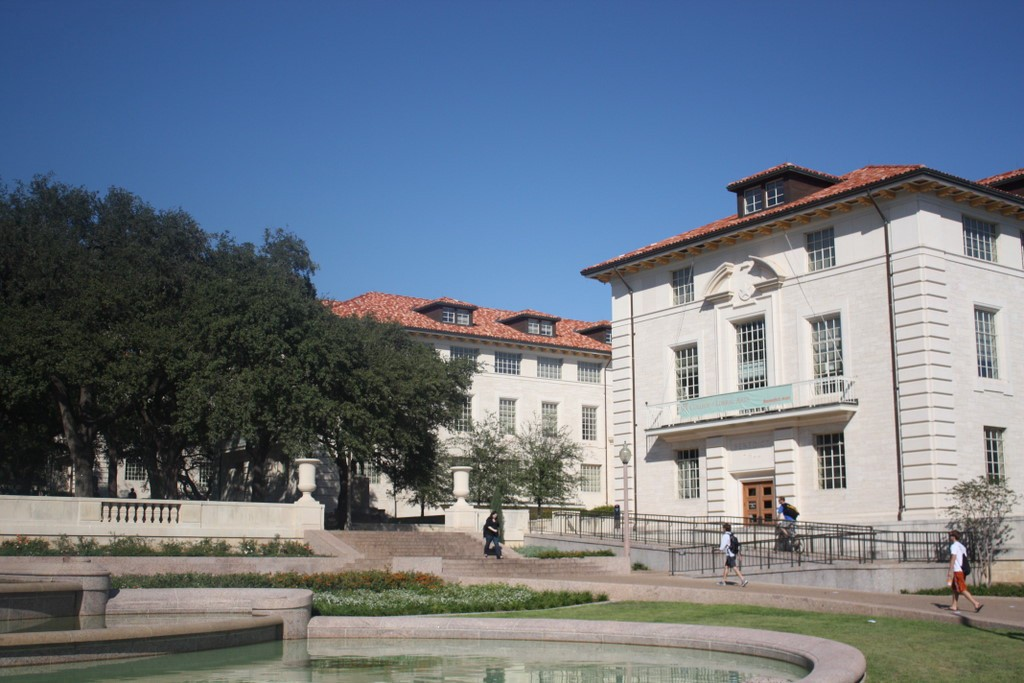
\includegraphics[height=3.6cm]{figures/foto1A.jpg}
\caption{foto1A.jpg} \label{foto1A}
\end{center}
\end{figure}

\begin{figure}[H]
\begin{center}
	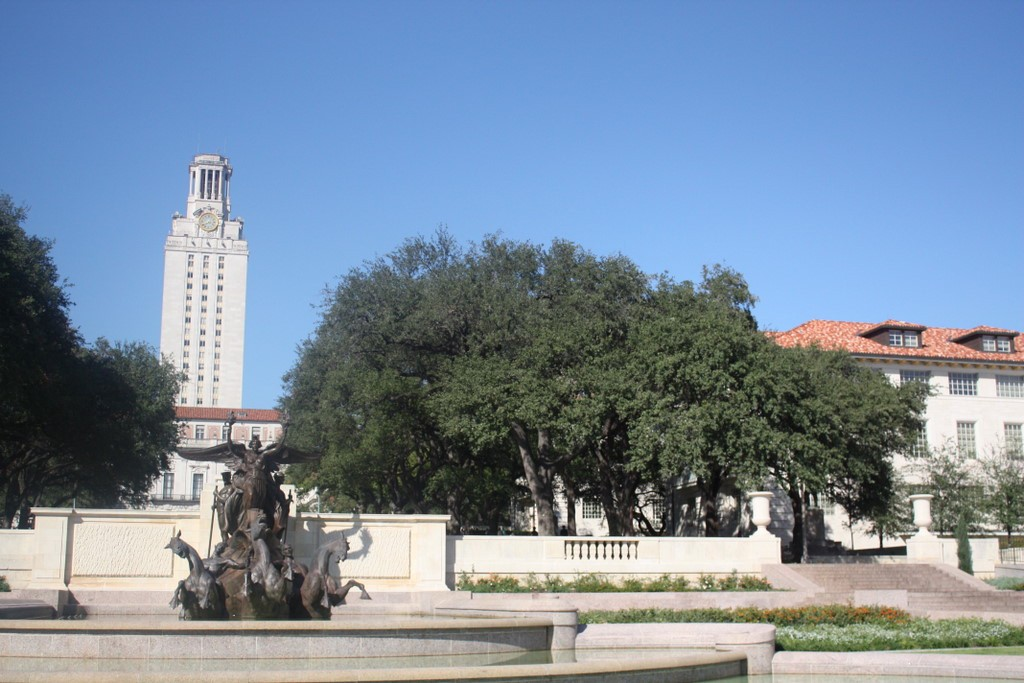
\includegraphics[height=3.6cm]{figures/foto1B.jpg}
\caption{foto1B.jpg} \label{foto1B}
\end{center}
\end{figure}

\begin{figure}[H]
\begin{center}
	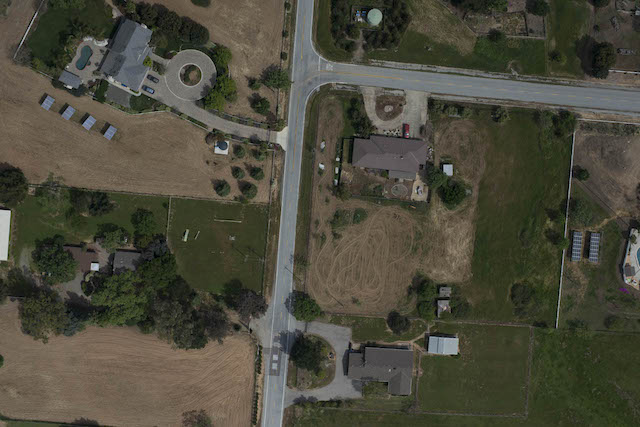
\includegraphics[height=3.6cm]{figures/foto3A.jpg}
\caption{foto3A.jpg} \label{foto3A}
\end{center}
\end{figure}

\begin{figure}[H]
\begin{center}
	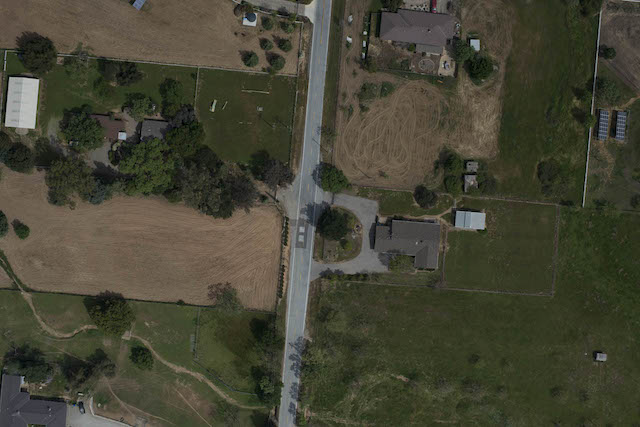
\includegraphics[height=3.6cm]{figures/foto3B.jpg}
\caption{foto3B.jpg} \label{foto3B}
\end{center}
\end{figure}

%------------------------------------------------

\section{Dependências e Códigos}

As bibliotecas utilizadas neste trabalho foram:

\begin{table}[H]
\begin{center}
\begin{tabular}{|l|l|}
\hline
\textbf{Biblioteca} & \textbf{Versão} \\ \hline
numpy               & 1.16.2          \\ \hline
cv2                 & 3.4.2           \\ \hline
matplotlib          & 3.0.3           \\ \hline
warnings            & 2.1             \\ \hline
\end{tabular}
\end{center}
\end{table}

A leitura das imagens foi realizada utilizando uma função do \textbf{matplotlib} \cite{b3} chamada \textbf{pyplot.imread()}, a qual nescessita apenas do caminho da imagem, já que queremos as informações das imagens assim como estão.

Foi criada uma função para plotar os resultados intermediários e finais utilizando também uma função do \textbf{matplotlib} chamada \textbf{pyplot.imshow()}. No passo (1) da descrição do trabalho foi utilizada uma função do \textbf{opencv} \cite{b1}, denominada \textbf{cv2.cvtColor()}, para transformar a imagem lida inicialmente em uma imagem em escala de cinza, para isso foi necessário a utilização da constante \textbf{cv2.COLOR\_BGR2GRAY}.

Para a utilização dos descritores pedidos no trabalho, foram utilizadas as funções do próprio \textbf{opencv}: \textit{SIFT} \textbf{cv2.xfeatures2d.SIFT\_create()}, \textit{SURF} \textbf{cv2.xfeatures2d.SURF\_create()}, \textit{BRIEF} \textbf{cv2.xfeatures2d.BriefDescriptorExtractor\_create()} e \textit{ORB} \textbf{cv2.ORB\_create()}.

No passo (3) e (4), como é necessário calcular a distância entre os \textit{keypoints} da imagens em questão e  utilizar somente os pontos que possuem uma melhor correspondência, utilizamos a função do \textbf{opencv} \textbf{knnMatch()} para fazer esse cálculo e uma taxa de $0.8$ para termos os pares de pontos que possuem correspondência válida.

No passo (5) é necessário o cálculo da matriz de homografia, como já sugerido na descrição, utilizamos a função \textbf{cv2.findHomography()} com a técnica \textit{RANSAC} (\textbf{cv2.RANSAC}) e um limiar de $4.0$. Para o cálculo da projeção de perspectiva foi utilizada a função \textbf{cv2.warpPerspective()} e, por fim, foram desenhadas as retas entre cada par de pontos que possuem uma maior similaridade.


%------------------------------------------------

\section{Fundamentação}

\subsection{Descritores}

Dada um imagem qualquer, pontos de interesse de um objeto pertencente a imagem podem ser extraídos para que se tenha uma descrição de características desse objeto. A seguir estão as descrições dos descritores utilizados nesse trabalho.

\subsubsection{SIFT}

O descritor SIFT (\textit{Scale-invariant feature transform}) é um algoritmo de detecção de características em Visão Computacional para detectar e descrever características locais em imagens. Um ponto de interesse SIFT é uma região de imagem circular com uma orientação. Ele é descrito por um quadro geométrico de quatro parâmetros: o centro do ponto-chave coordena $x$ e $y$, sua escala (o raio da região) e sua orientação (um ângulo expresso em radianos). O detector SIFT usa como estruturas de imagem de pontos chave que se assemelham a ''blobs''. Ao procurar por blobs em várias escalas e posições, o detector SIFT é invariante (ou, mais precisamente, covariante) para translação, rotações e redimensionamento da imagem.

\subsubsection{SURF}

O descritor SURF (\textit{Speeded up robust features}) é um detector e descritor de características locais patenteado. Pode ser usado para tarefas como reconhecimento de objetos, registro de imagens, classificação ou reconstrução 3D.

Para detectar pontos de interesse, o SURF usa uma aproximação inteira do determinante do detector de \textit{blob Hessian}, que pode ser calculado com 3 operações inteiras usando uma imagem integral pré-calculada. Seu descritor de característica é baseado na soma da resposta da \textit{wavelet Haar} em torno do ponto de interesse. Estes também podem ser calculados com o auxílio da imagem integral.

\subsubsection{BRIEF}

O descritor BRIEF (\textit{Binary Robust Independent Elementary Features}) fornece um atalho para encontrar as cadeias binárias diretamente, sem encontrar descritores. Dado uma imagem, ele seleciona um conjunto de pares de localizações $n_{d}(x,y)$ em um único caminho. Então, algumas comparações de intensidade de \textit{pixels} são realizadas nesses pares de localizações. Por exemplo, suponha dois pares de localizações $p$ e $q$, se $I(p) < I(q)$, então o resultado é 1, se não, o resultado é 0. Isso é aplicado para todos os pares de localizações para obter uma string binária $n_{d}-$dimensional. E, assim, realizar os cálculos dos pontos de interesse.

\subsubsection{ORB}

O descritor ORB (\textit{Oriented FAST and rotated BRIEF}) é um detector rápido de características locais. É baseado no detector de pontos de interesse FAST e no descritor visual BRIEF. Seu objetivo é fornecer uma alternativa rápida e eficiente para o SIFT.

\subsection{RANSAC}

RANSAC é uma abreviatura de ''\textit{RANdom SAmple Consensus}''. É um método iterativo para estimar os parâmetros de um modelo matemático \cite{b4}.

Dado um modelo que requer um mínimo de $n$ pontos para instanciar seus parametros livres, e um conjunto de pontos $P$, tal que o numero de pontos em $P$ é maior que $n$, seleciona randomicamente um subconjunto $S_{1}$ de $n$ pontos de $P$ e instancia o modelo. Usa-se o modelo instanciado $M_{1}$ para determinar o subconjunto $S_{1}*$ de pontos em $P$ que estão dentro de um erro tolerável de $M_{1}$. O conjunto $S_{1}*$ é chamado de conjunto consenso de $S_{1}$.

Se o número de elementos de $S_{1}*$ é maior que certo limite $t$, que é função da estimativa do número de erros grosseiros em $P$, usar $S_{1}*$ para computar (possivelmente com Mínimos Quadrados) um novo modelo $M_{1}*$.

Se o número de elementos de $S_{1}*$ é menor do que $t$, seleciona-se randomicamente um novo subconjunto $S_{2}$ e repete-se o processo acima. Se, após um número pré determinado de tentativas, nenhum conjunto consenso com $t$ ou mais membros tiver sido encontrado, ou soluciona-se o modelo com o maior conjunto consenso, ou termina-se com falha.

%------------------------------------------------

\section{Saída de Dados}

As imagens resultantes foram salvas dentro da pasta \textbf{resultados/} utilizando uma função da biblioteca \textbf{matplotlib} chamada \textbf{pyplot.imsave()} \cite{b3}.

O formato dos nomes de saída estão da seguinte forma: as imagens que representam as projeções de perspectiva possuem os nomes ''descritor\_persp\_inter\_nomedafoto.jpeg''; as imagens que representam as junções das projeções de perspectiva possuem os nomes ''descritor\_persp\_nomedafoto.jpeg''; e, por fim, as imagens que represenção as projeções de perspectiva com as retas de correspondências desenhadas possuem os nomes ''descritor\_vis\_nomedafoto.jpeg''.

%------------------------------------------------

\section{Resultados e Discuções}

Os resultados obtidos com a aplicação do passo a passo definido no problema estão a seguir:

\begin{figure}[H]
\begin{center}
	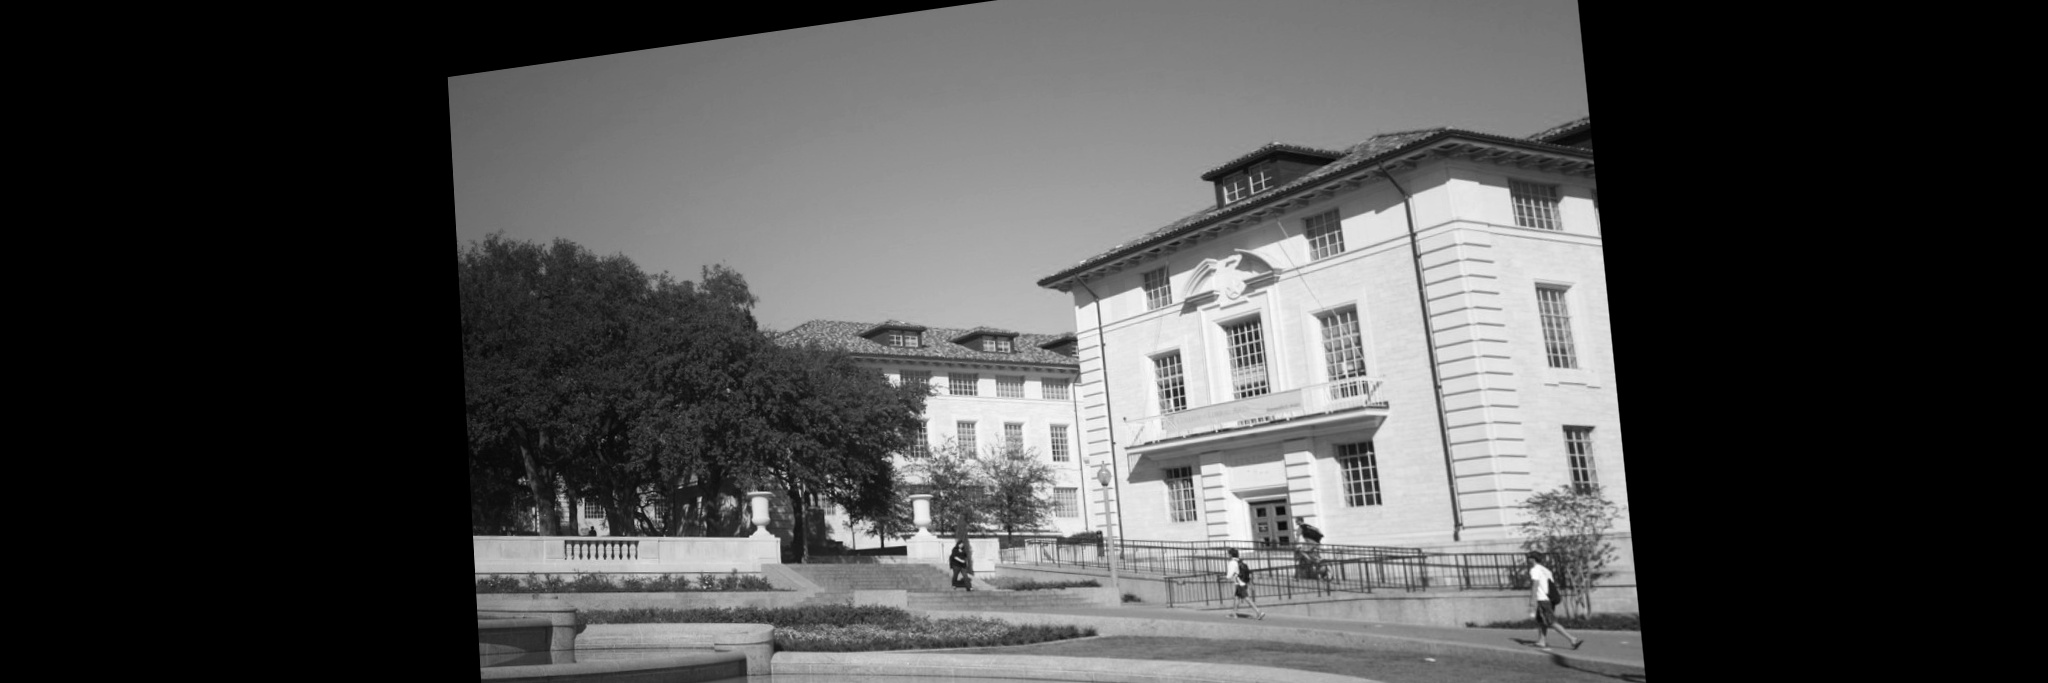
\includegraphics[width=7cm]{figures/sift_persp_inter_foto1.jpeg}
\caption{sift\_persp\_inter\_foto1.jpeg} \label{sift_persp_inter_foto1}
\end{center}
\end{figure}

A Figura~\ref{sift_persp_inter_foto1} apresenta o resultado do passo (6), o qual é necessário aplicar uma projeção de perspectiva para alinhar as imagens. Essa figura mostra como ficou o resultado da imagem que foi transformada com base nos pontos que foram obtidos com o descritor \textit{SIFT}. Podemos destacar que a imagem sofre uma transformação não linear, com uma pequena rotação para que pudesse ficar se assemelhar a continuidade da imagem 1.

\begin{figure}[H]
\begin{center}
	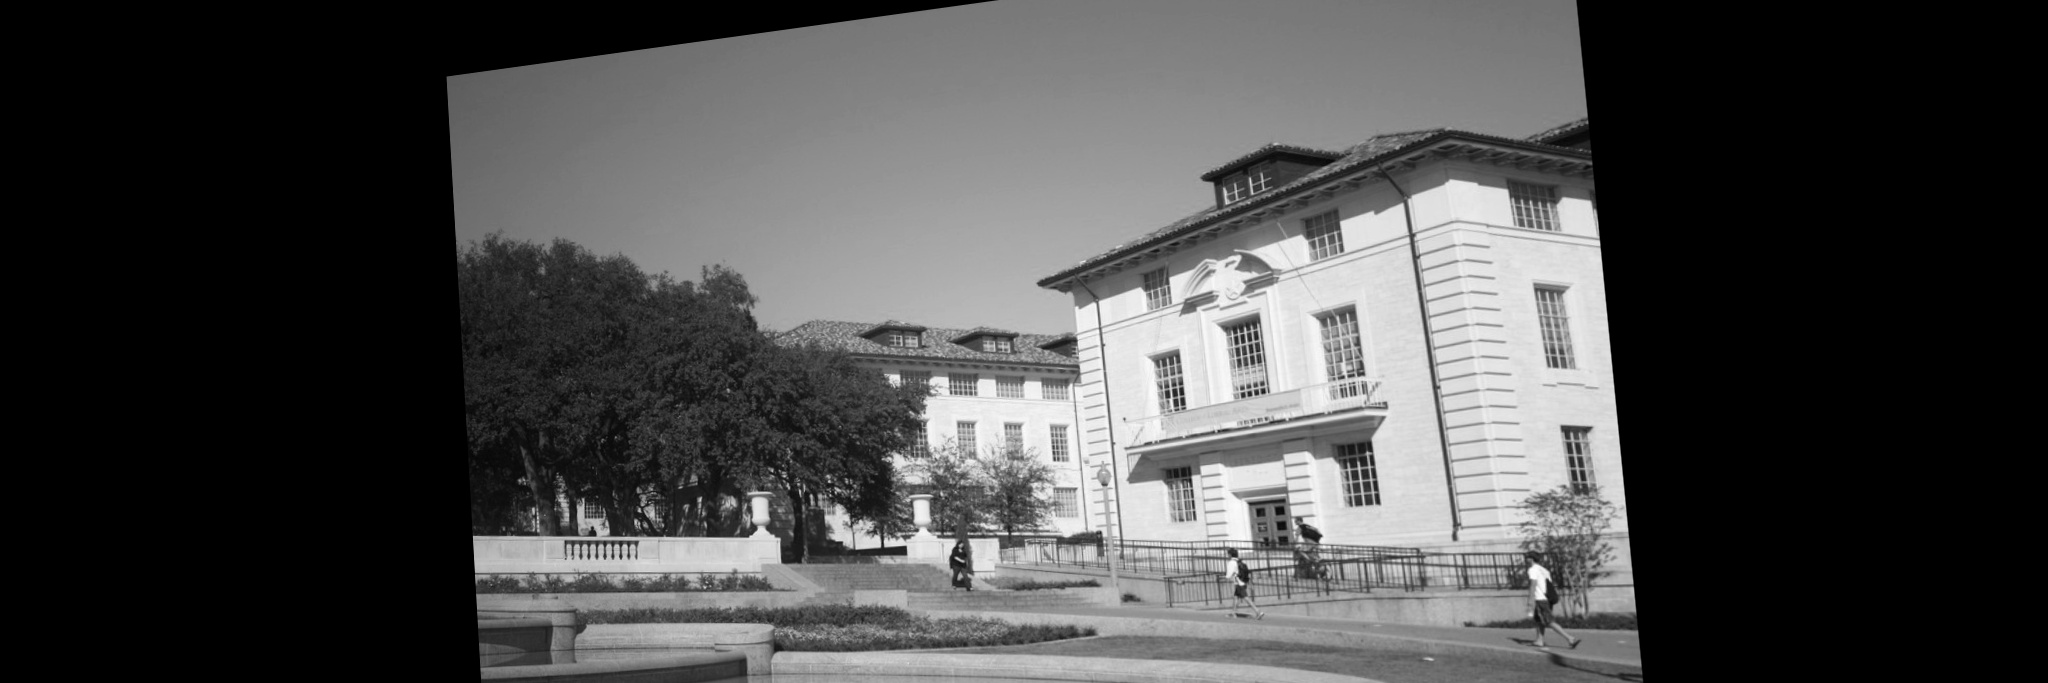
\includegraphics[width=7cm]{figures/surf_persp_inter_foto1.jpeg}
\caption{surf\_persp\_inter\_foto1.jpeg} \label{surf_persp_inter_foto1}
\end{center}
\end{figure}

A Figura~\ref{surf_persp_inter_foto1} aprensenta também o resultado obtido após o passo (6), porém, com o descritor \textit{SURF}. Podemos destacar que os resultados foram parecidos com a imagem anterior e que a imagem resultante sofreu, praticamente, as mesmas transformações.

\begin{figure}[H]
\begin{center}
	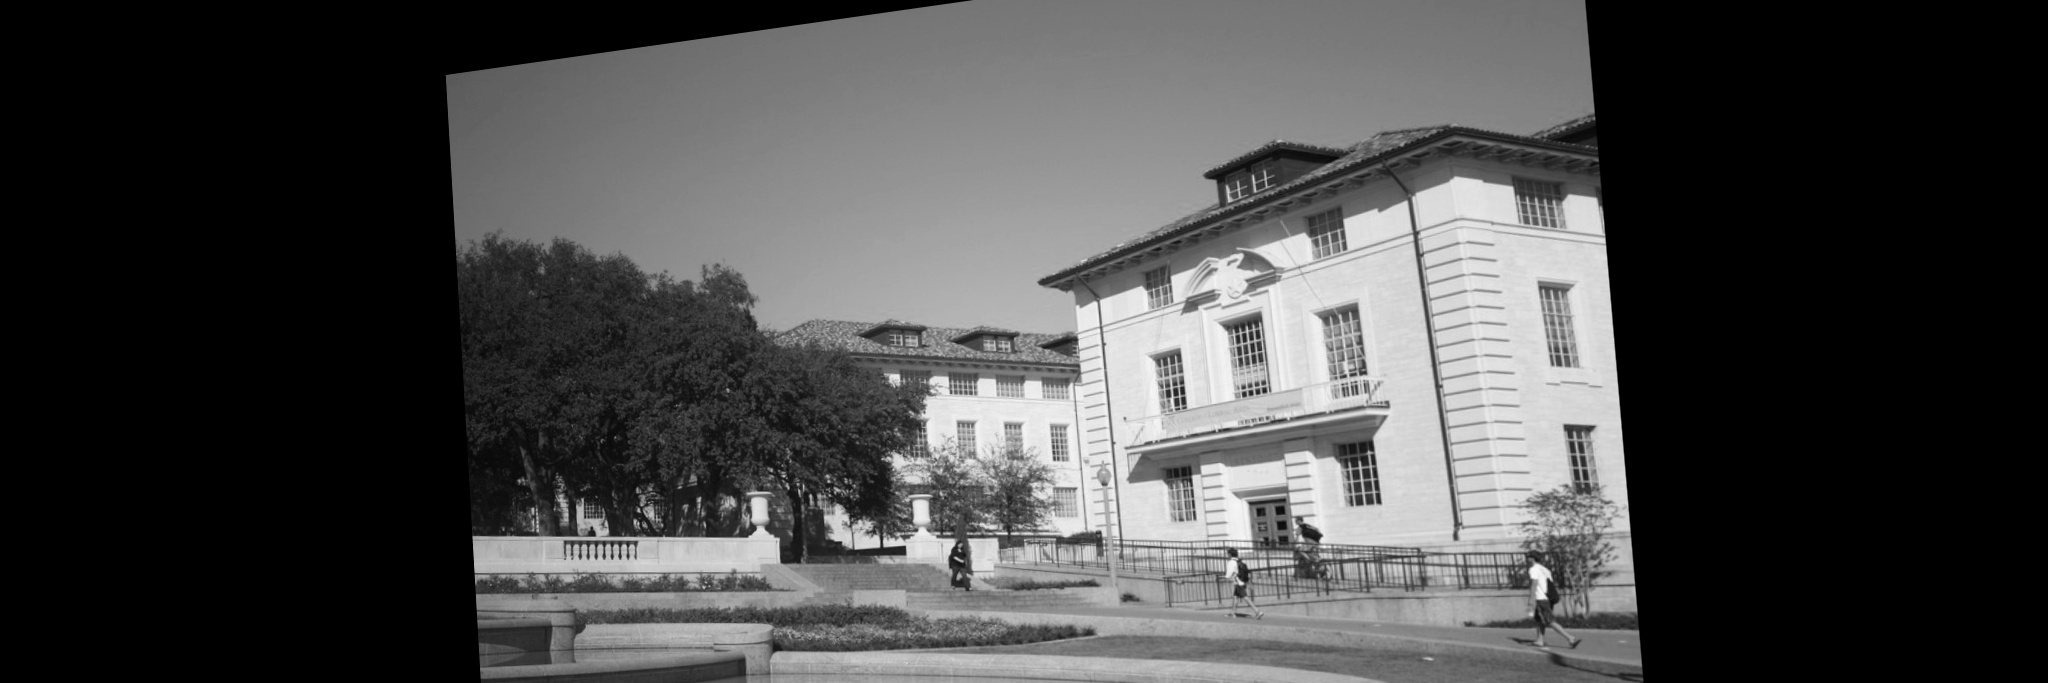
\includegraphics[width=7cm]{figures/brief_persp_inter_foto1.jpeg}
\caption{brief\_persp\_inter\_foto1.jpeg} \label{brief_persp_inter_foto1}
\end{center}
\end{figure}

A Figura~\ref{brief_persp_inter_foto1} apresenta o resultado obtido após o passo (6), mas utilizando os pontos de interesse obtidos com o descritor \textit{BRIEF}. Assim como as duas imagens anteriores, os resultados foram bem semelhantes e sofreram, visualmente, as mesmas transformações.

\begin{figure}[H]
\begin{center}
	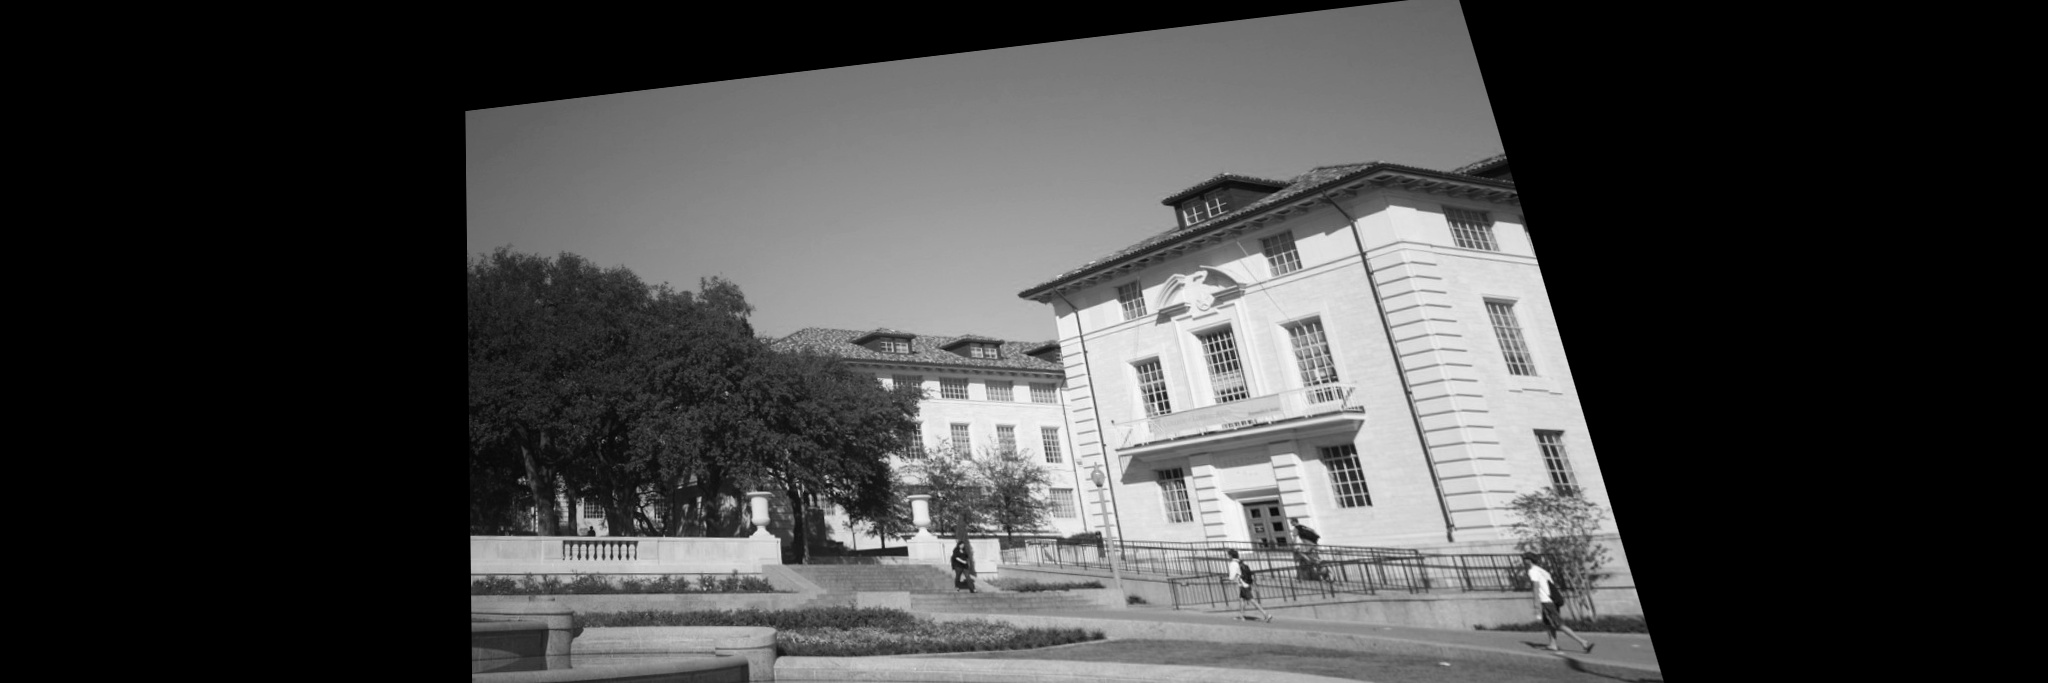
\includegraphics[width=7cm]{figures/orb_persp_inter_foto1.jpeg}
\caption{orb\_persp\_inter\_foto1.jpeg} \label{orb_persp_inter_foto1}
\end{center}
\end{figure}

A Figura~\ref{orb_persp_inter_foto1} mostra o resultado obtido após o passo (6) também, porém, utilizando os pontos de interesse resultantes da aplicação do descritor \textit{ORB}. Podemos observar que a imagem não se assemelha as anteriores, o que é causado pelo fato de o descritor \textit{ORB} ter resultado em uma quantidade consideravelmente diferente de pontos de interesse dos descritores aplicados anteriormente. Assim, essa figura sofreu transformações diferentes, o que vai ficar claro na execução do passo (7).

\begin{figure}[H]
\begin{center}
	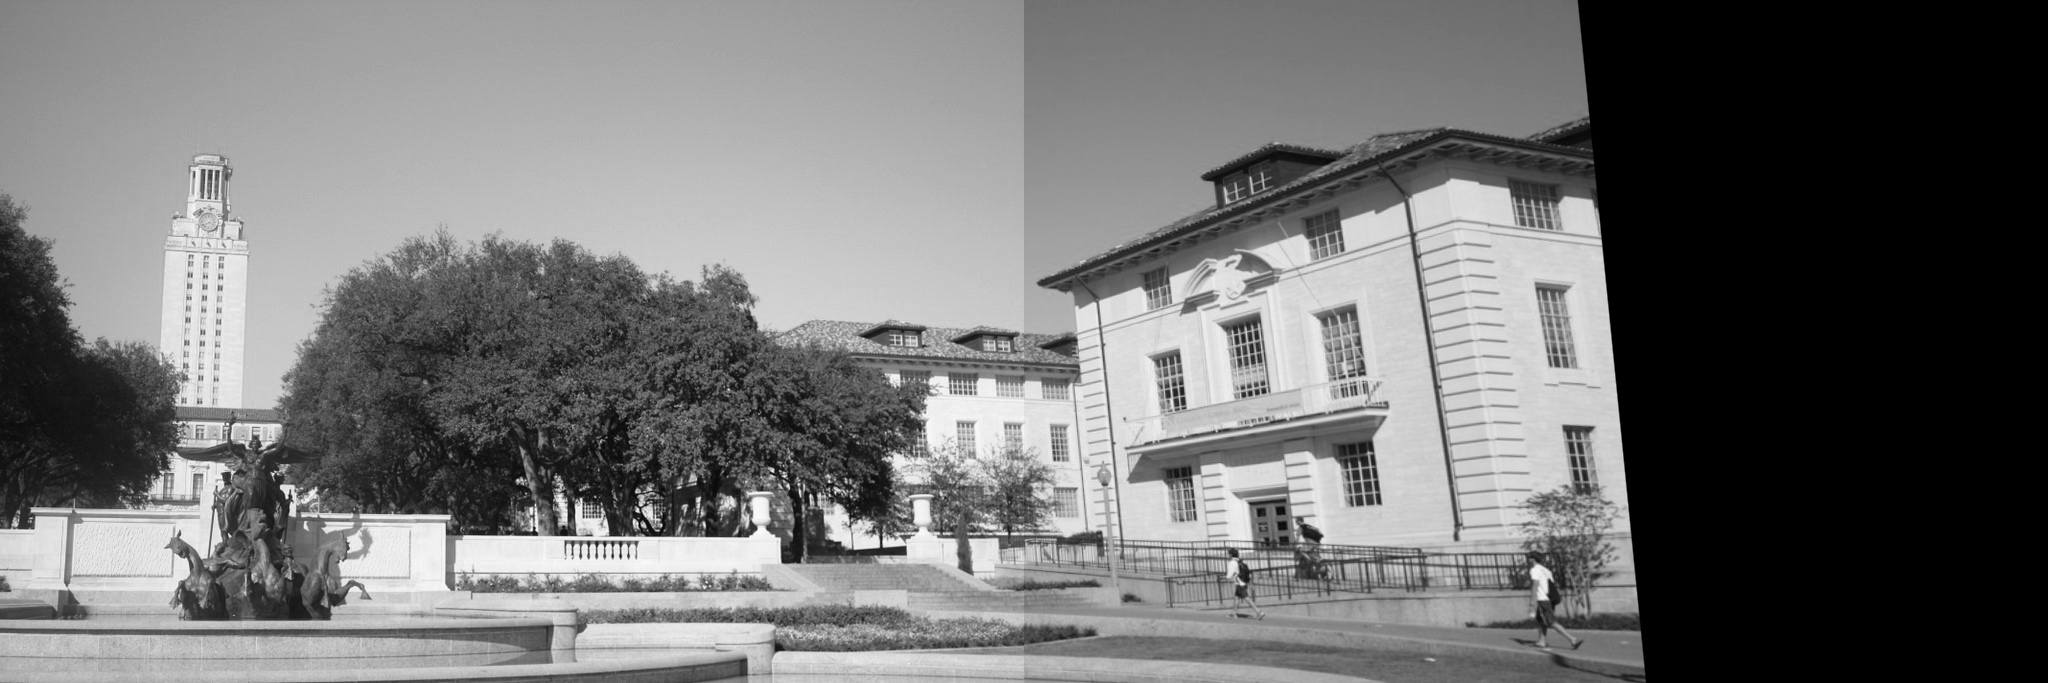
\includegraphics[width=7cm]{figures/sift_persp_foto1.jpeg}
\caption{sift\_persp\_foto1.jpeg} \label{sift_persp_foto1}
\end{center}
\end{figure}

A Figura~\ref{sift_persp_foto1} mostra o resultado da aplicação do passo (7), o qual é necessário unir as imagens alinhadas e criar a imagem panorâmica a partir disso. Podemos observar que o resultado foi satisfatório, as imagens se alinharam muito bem na ''linha de intersecção'' e formaram uma imagem panorâmica assim como é descrito no passo (7). 

\begin{figure}[H]
\begin{center}
	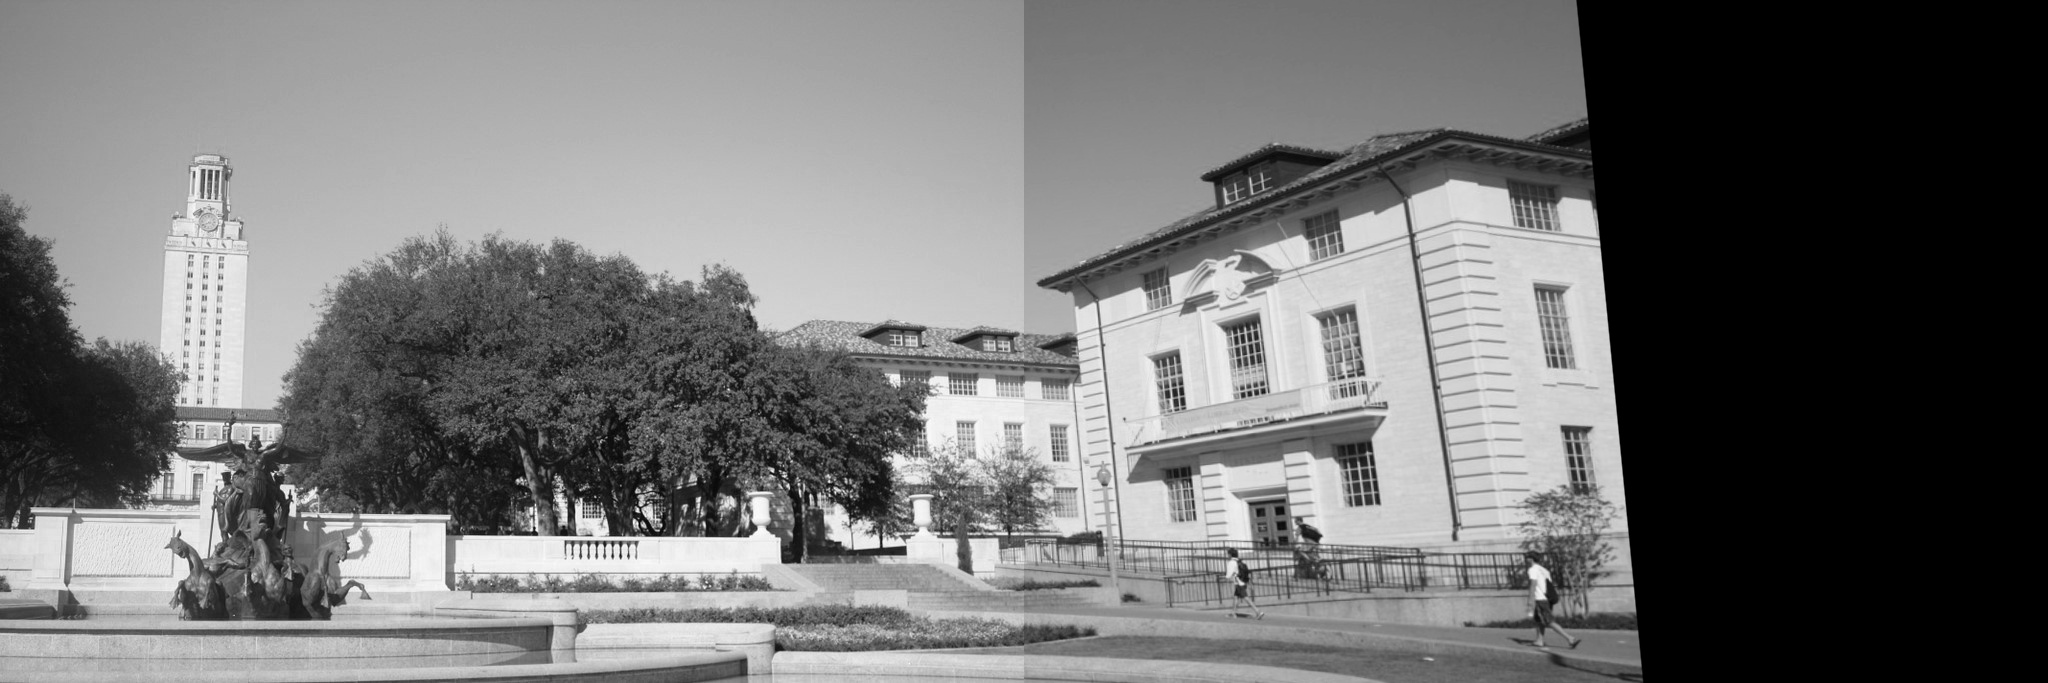
\includegraphics[width=7cm]{figures/surf_persp_foto1.jpeg}
\caption{surf\_persp\_foto1.jpeg} \label{surf_persp_foto1}
\end{center}
\end{figure}

A Figura~\ref{surf_persp_foto1} apresenta o resultado obtido após a execução do passo (7), mas com a utilização do descritor \textit{SURF}. Podemos destacar que assim como visto nos resultados do passo (6), os descritores \textit{SIFT} e \textit{SURF} descrevam pontos semelhantes e, por tanto, as transformações aplicadas nas imagens também foram parecidos, o que resultou em imagens panorâmicas semelhantes também.

\begin{figure}[H]
\begin{center}
	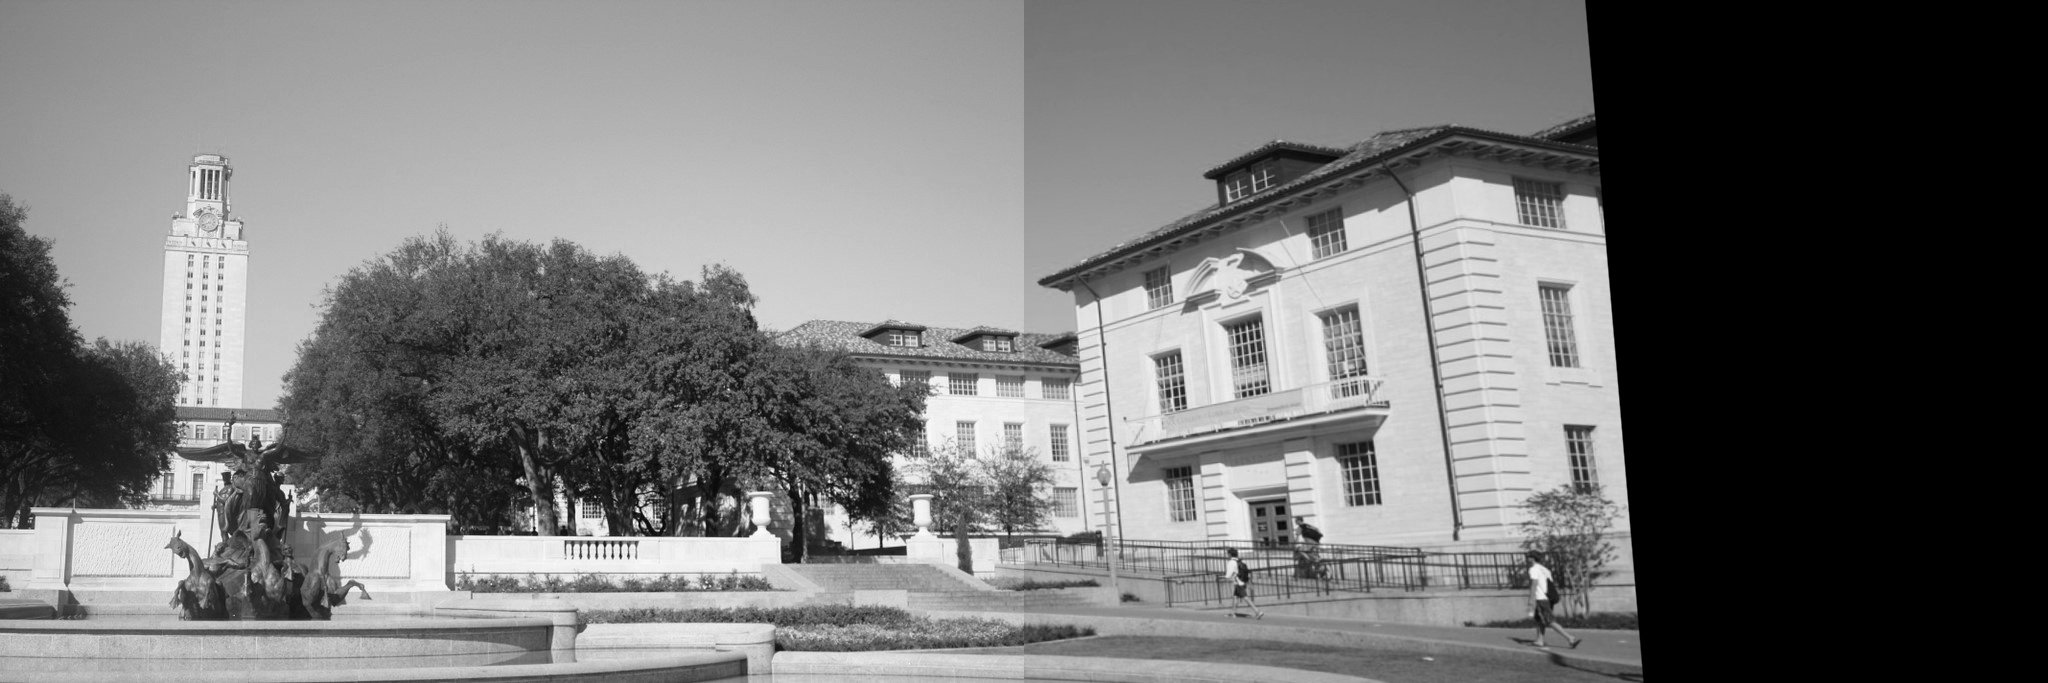
\includegraphics[width=7cm]{figures/brief_persp_foto1.jpeg}
\caption{brief\_persp\_foto1.jpeg} \label{brief_persp_foto1}
\end{center}
\end{figure}

A Figura~\ref{brief_persp_foto1} mostra também o resultado obtido após a execução do passo (7), porém, com a utilização do descritor \textit{BRIEF} para descrever os pontos de interesse nas imagens. Assim como nas duas imagens anteriores, o resultado da imagem panorâmica foi bem parecido, o que reforça a questão dos descritores terem escolhidos pontos de interesse semelhantes.

\begin{figure}[H]
\begin{center}
	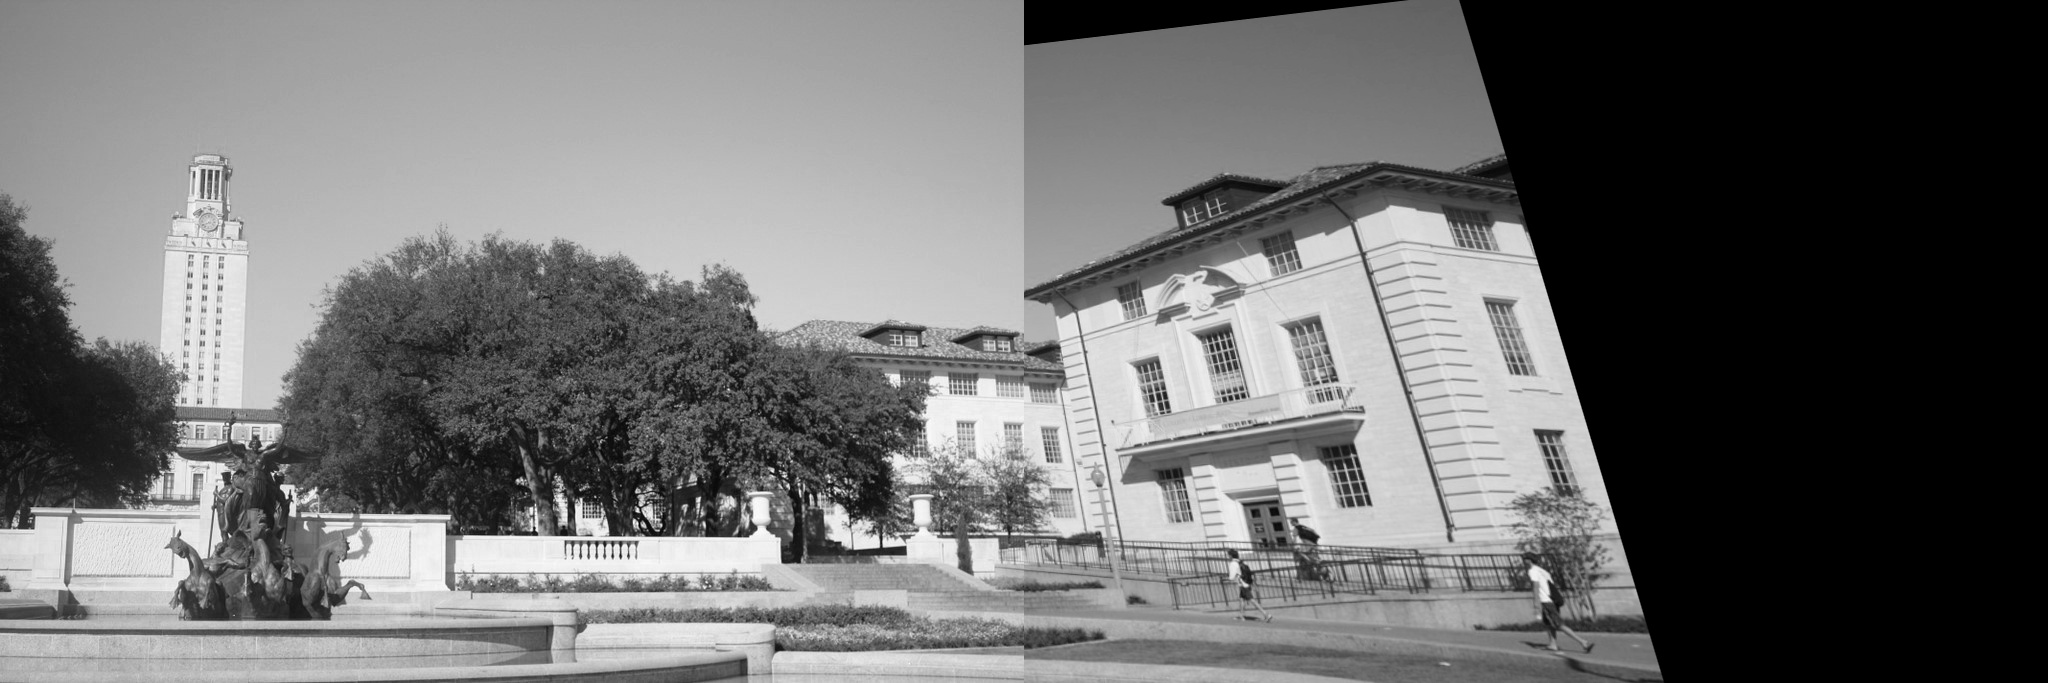
\includegraphics[width=7cm]{figures/orb_persp_foto1.jpeg}
\caption{orb\_persp\_foto1.jpeg} \label{orb_persp_foto1}
\end{center}
\end{figure}

Como última figura do passo (7), a Figura~\ref{orb_persp_foto1} apresenta o resultado da imagem panorâmica utilizando o descritor \textit{ORB} para definir os pontos de interesse. Podemos ver algumas falhas em comparação com as desmais imagens panorâmicas, isso se deve ao fato da grande diferença de detecção de pontos de interesse entre o descritor \textit{ORB} e os demais descritores, como será evidenciado a seguir. 

\begin{figure}[H]
\begin{center}
	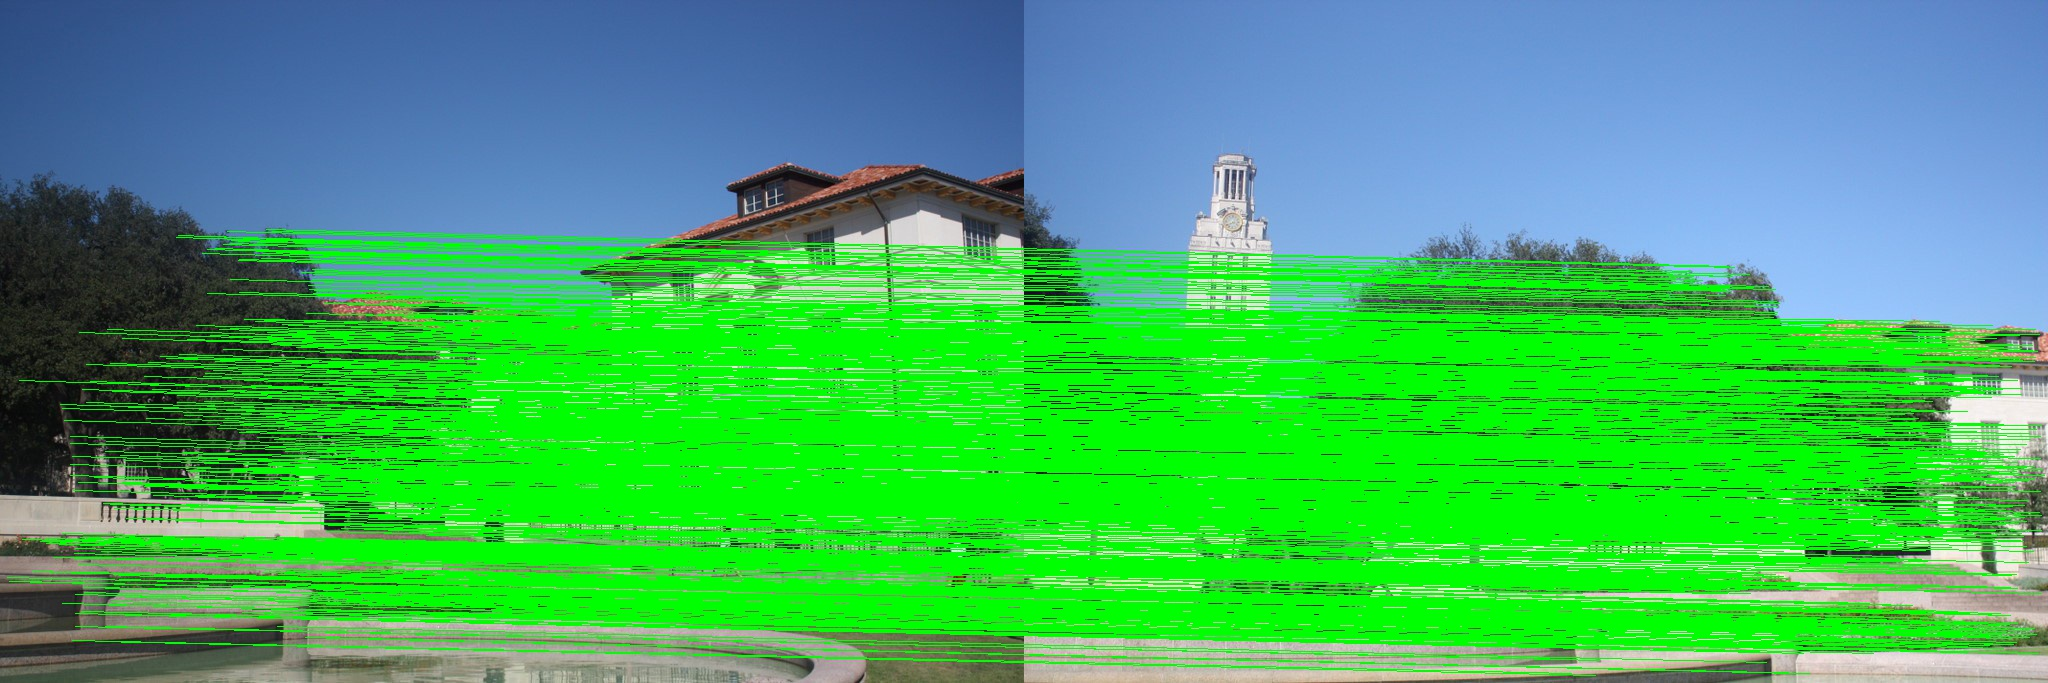
\includegraphics[width=7cm]{figures/sift_vis_foto1.jpeg}
\caption{sift\_vis\_foto1.jpeg} \label{sift_vis_foto1}
\end{center}
\end{figure}

Na Figura~\ref{sift_vis_foto1} podemos ver o resultado do passo (8), o qual é necessário desenhar as retas entre os pontos correspondentes no par de imagens em questão. Podemos destacar que o descritor \textit{SIFT} conseguiu detectar uma grande quantidade de pontos de interesse nas duas imagens e, com isso, obteve um ótimo resultado quando aplicado nessas imagens de entrada. Vale destacar também que, como os pontos de interesse não estão concentrados em uma mesma região, pode-se obter melhores resultados no passo de geração da projeção em perspectiva.

\begin{figure}[H]
\begin{center}
	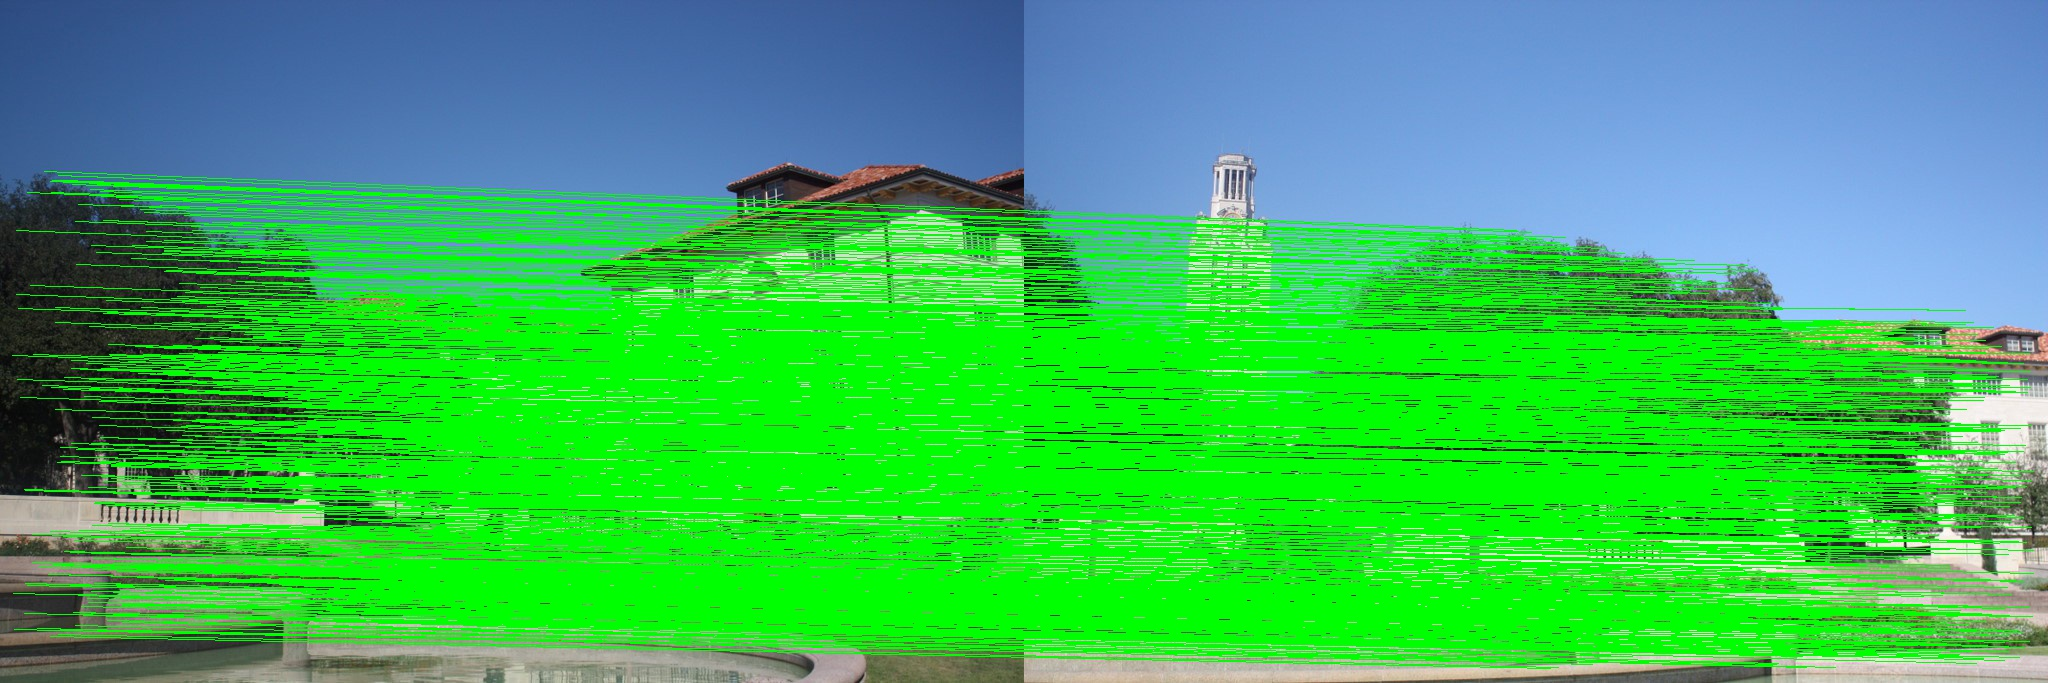
\includegraphics[width=7cm]{figures/surf_vis_foto1.jpeg}
\caption{surf\_vis\_foto1.jpeg} \label{surf_vis_foto1}
\end{center}
\end{figure}

A Figura~\ref{surf_vis_foto1} apresenta também o resultado do passo (8), porém, utilizando o descritor \textit{SURF} para obter os pontos de interesse. Assim como na imagem referente ao descritor \textit{SIFT}, essa figura mostra que o descritor \textit{SURF} conseguiu detectar uma grande quantidade de pontos de interesse e em diferentes regiões das imagens. Podemos dizer que esses dois descritores se mostraram equivalentes quando aplicados a essas imagens de entrada.

\begin{figure}[H]
\begin{center}
	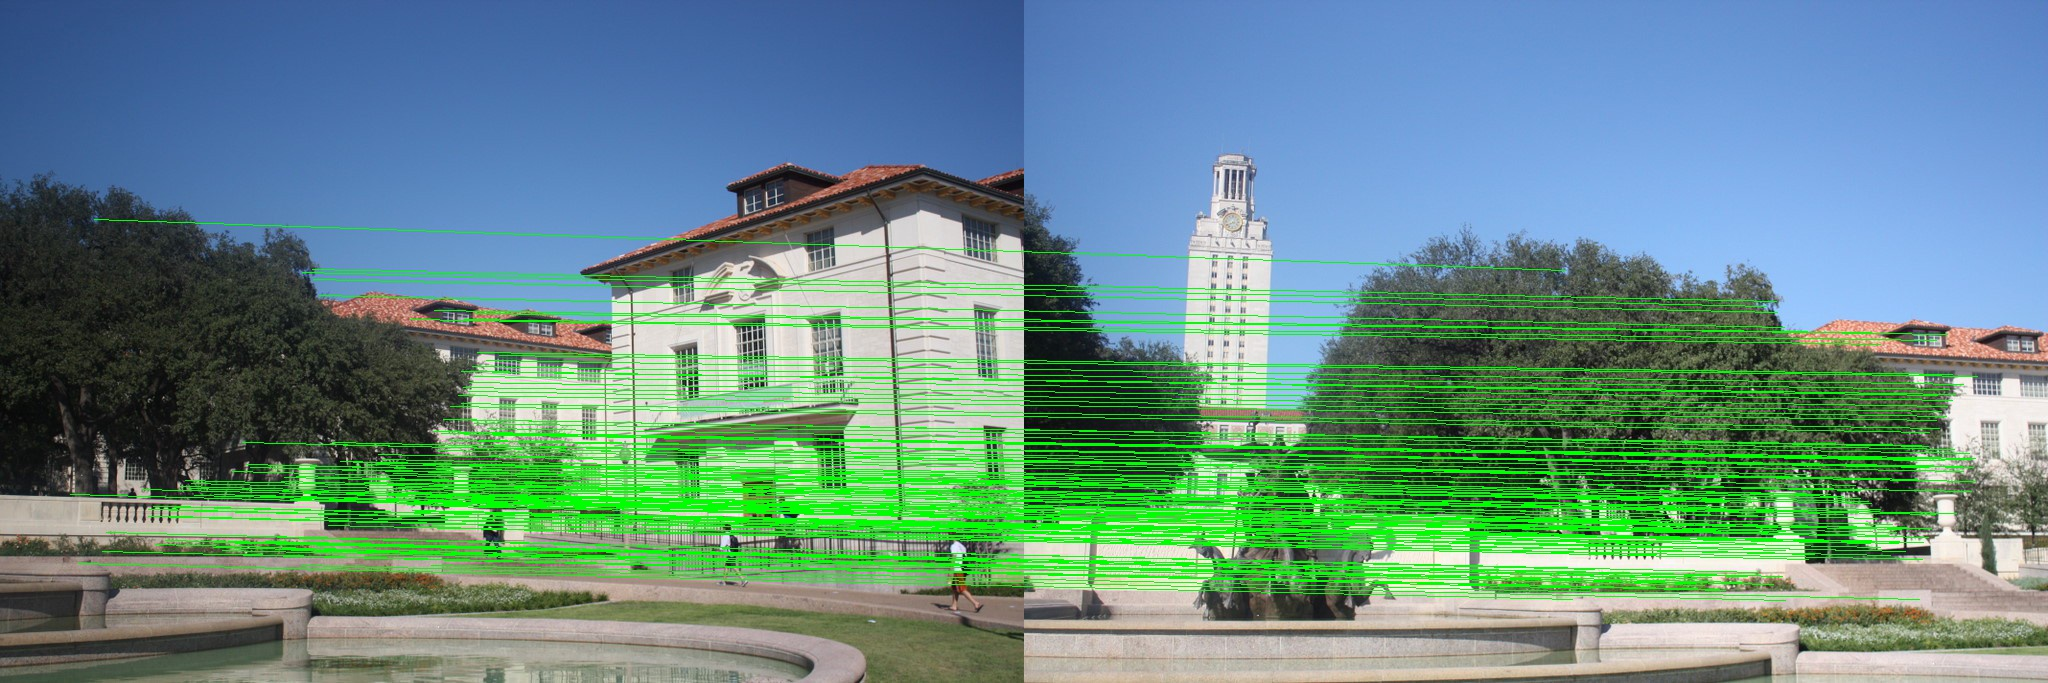
\includegraphics[width=7cm]{figures/brief_vis_foto1.jpeg}
\caption{brief\_vis\_foto1.jpeg} \label{brief_vis_foto1}
\end{center}
\end{figure}

A Figura~\ref{brief_vis_foto1} apresenta o resultado do passo (8) utilizando como descritor o \textit{BRIEF}. Podemos observar que foi detectado uma quantidade bem menor de pontos de interesse, quando comparado ao \textit{SIFT} e \textit{SURF}, porém os pontos de interesse detectados são bem diversificados em regiões da imagem, o que faz com que o resultado seja equivalente aos descritores anteriores.

\begin{figure}[H]
\begin{center}
	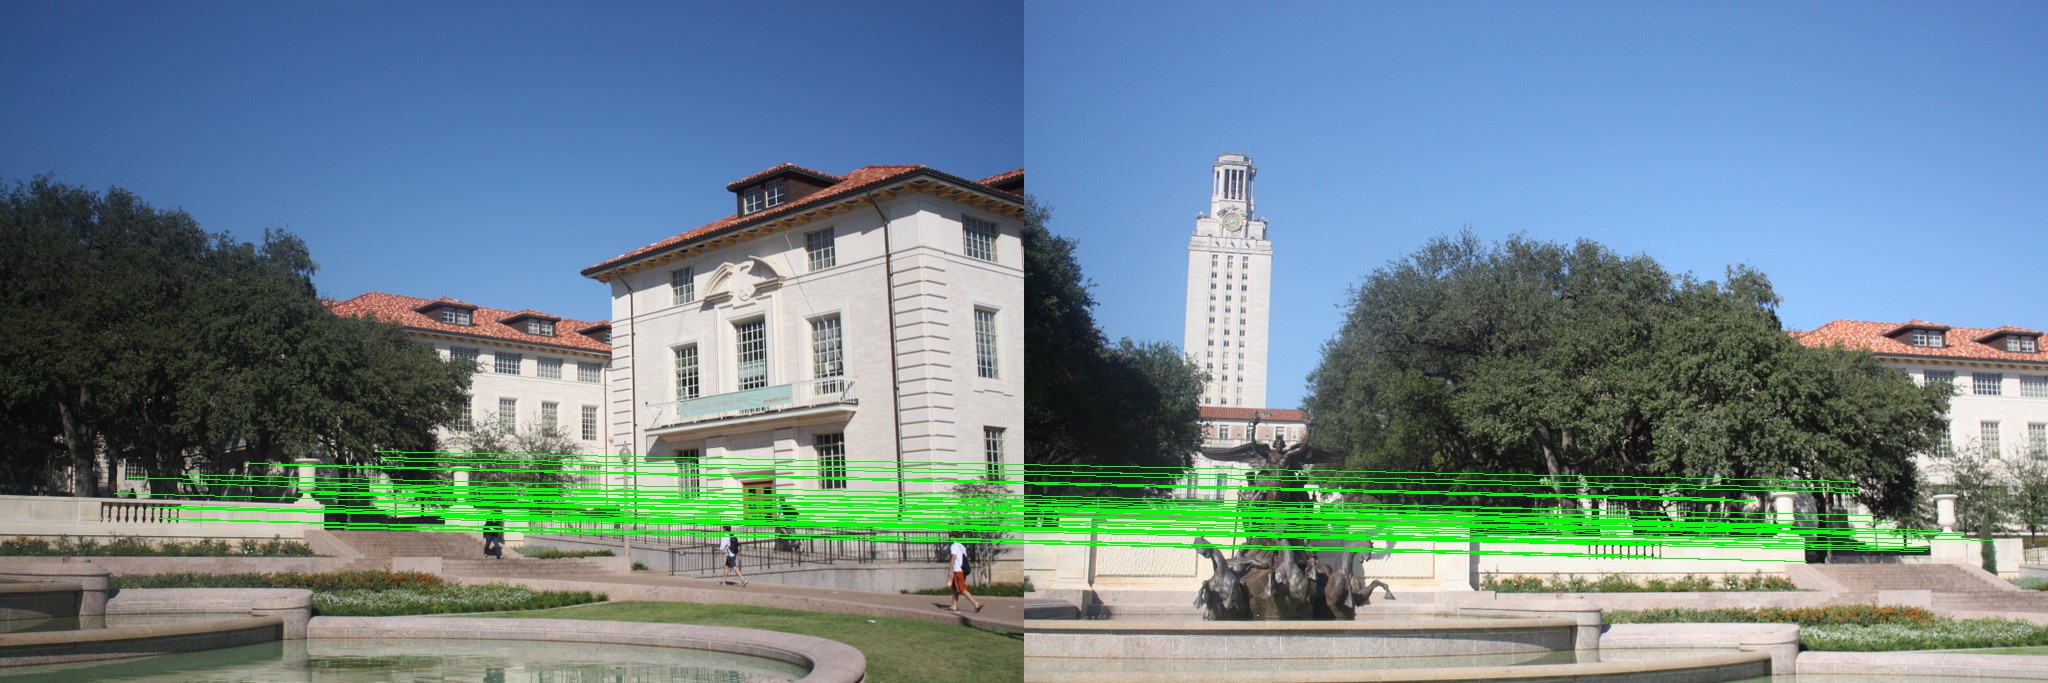
\includegraphics[width=7cm]{figures/orb_vis_foto1.jpeg}
\caption{orb\_vis\_foto1.jpeg} \label{orb_vis_foto1}
\end{center}
\end{figure}

A Figura~\ref{orb_vis_foto1} apresenta o resultado do passo (8), mas utilizando o descritor \textit{ORB} para detectar os pontos de interesse. Podemos observar que foi o descritor que obteve a menor quantidade de pontos de interesse e todos eles em uma mesma região da imagem, o que prejudica quando é necessário fazer a projeção de perspectiva do passo (6). Com isso, podemos ver que o resultado obtido com esse descritor é inferior quando comparado aos demais.

%------------------------------------------------

\section{Conclusão}

Podemos concluir que os resultados obtidos com as aplicações das técnicas de descrição de imagens e definição dos pontos de interesses nas imagens para a criação da imagem panorâmica e o traçado das retas entre os pontos de interesse foram satisfatórios quanto a especificação do trabalho e se mostrou razoável para este objetivo, assim, consolida ainda mais os conceitos vistos em sala de aula.

%----------------------------------------------------------------------------------------
%	REFERENCE LIST
%----------------------------------------------------------------------------------------

\begin{thebibliography}{99} % Bibliography - this is intentionally simple in this template

\bibitem{b1} Welcome to opencv documentation! \href{https://docs.opencv.org/2.4/index.html}{https://docs.opencv.org/2.4/index.html} Acesso em: 08/06/2019.

\bibitem{b2} Pedrini, Hélio, and William Robson Schwartz. Análise de imagens digitais: princípios, algoritmos e aplicações. Thomson Learning, 2008.

\bibitem{b3} Matplotlib Version 3.0.3 \href{https://matplotlib.org/contents.html}{https://matplotlib.org/contents.html} Acesso em: 08/06/2019.

\bibitem{b4} Wikipedia: RANSAC \href{https://pt.wikipedia.org/wiki/RANSAC}{https://pt.wikipedia.org/wiki/RANSAC} Acesso em: 08/06/2019.
 
\end{thebibliography}

%----------------------------------------------------------------------------------------

\section*{Anexos}

\begin{figure}[H]
\begin{center}
	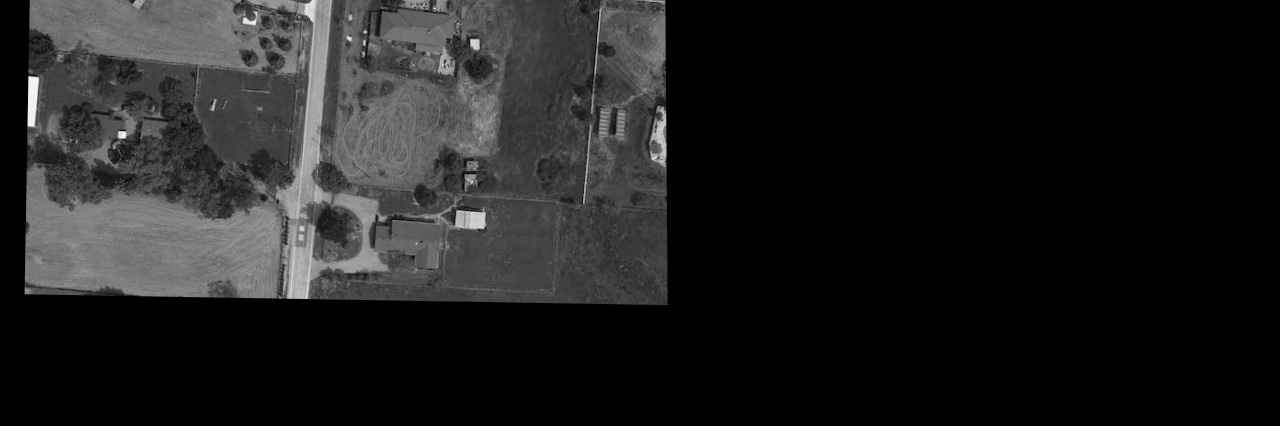
\includegraphics[width=7cm]{figures/sift_persp_inter_foto2.jpeg}
\caption{sift\_persp\_inter\_foto2.jpeg} \label{sift_persp_inter_foto2}
\end{center}
\end{figure}

\begin{figure}[H]
\begin{center}
	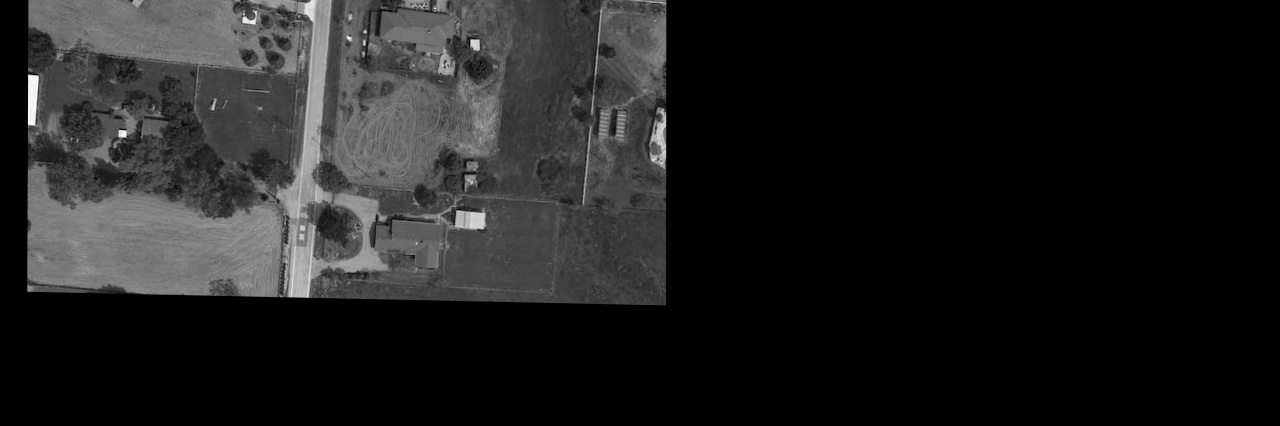
\includegraphics[width=7cm]{figures/surf_persp_inter_foto2.jpeg}
\caption{surf\_persp\_inter\_foto2.jpeg} \label{surf_persp_inter_foto2}
\end{center}
\end{figure}

\begin{figure}[H]
\begin{center}
	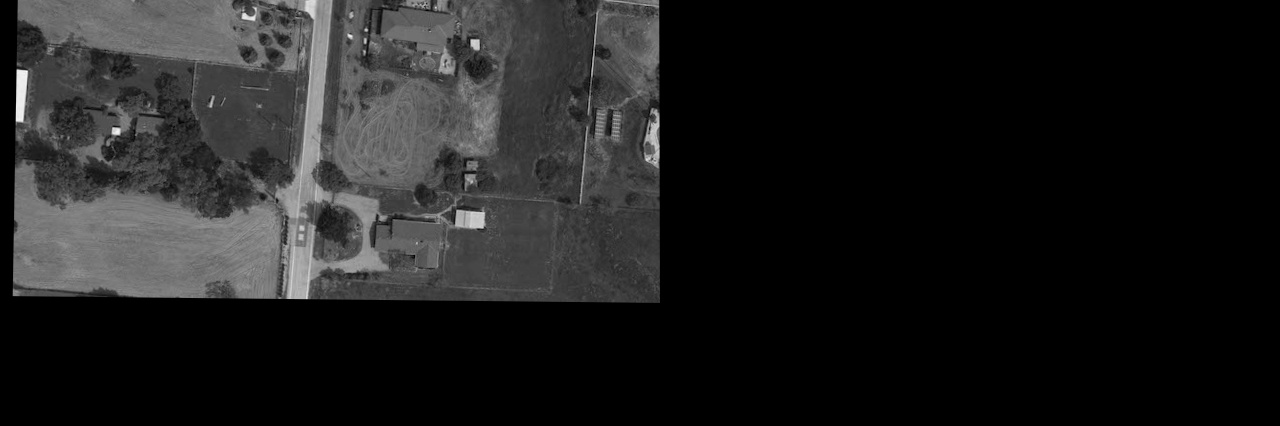
\includegraphics[width=7cm]{figures/brief_persp_inter_foto2.jpeg}
\caption{brief\_persp\_inter\_foto2.jpeg} \label{brief_persp_inter_foto2}
\end{center}
\end{figure}

\begin{figure}[H]
\begin{center}
	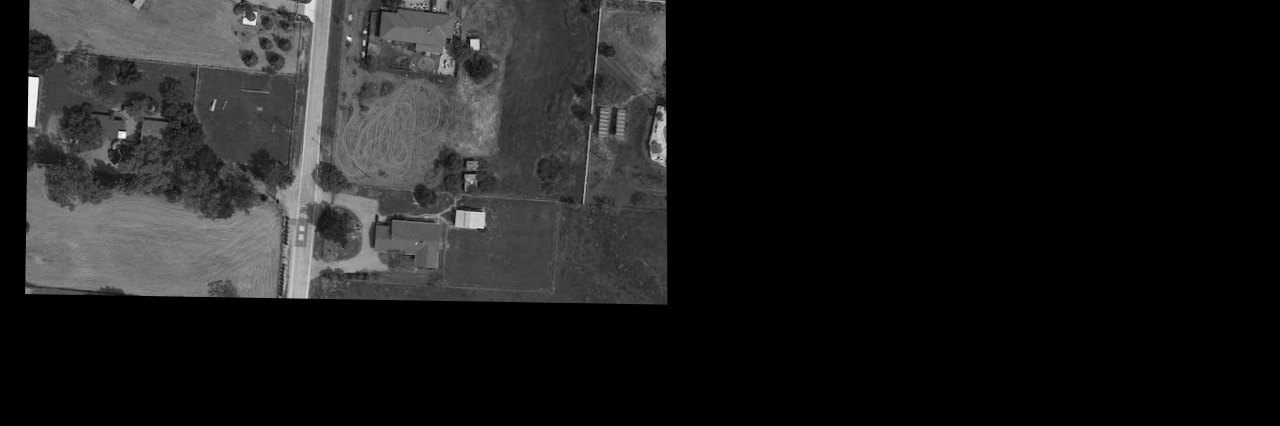
\includegraphics[width=7cm]{figures/orb_persp_inter_foto2.jpeg}
\caption{orb\_persp\_inter\_foto2.jpeg} \label{orb_persp_inter_foto2}
\end{center}
\end{figure}

\begin{figure}[H]
\begin{center}
	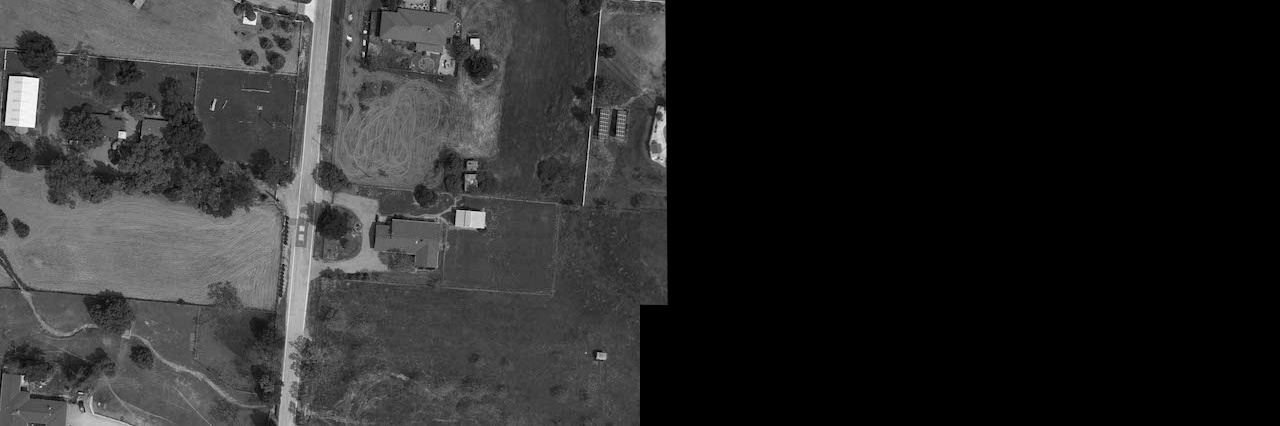
\includegraphics[width=7cm]{figures/sift_persp_foto2.jpeg}
\caption{sift\_persp\_foto2.jpeg} \label{sift_persp_foto2}
\end{center}
\end{figure}

\begin{figure}[H]
\begin{center}
	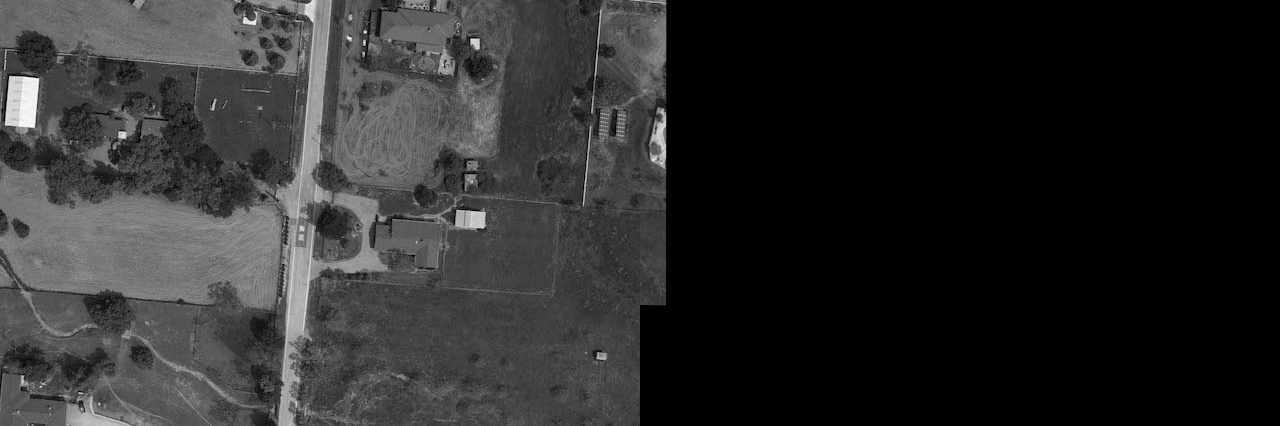
\includegraphics[width=7cm]{figures/surf_persp_foto2.jpeg}
\caption{surf\_persp\_foto2.jpeg} \label{surf_persp_foto2}
\end{center}
\end{figure}

\begin{figure}[H]
\begin{center}
	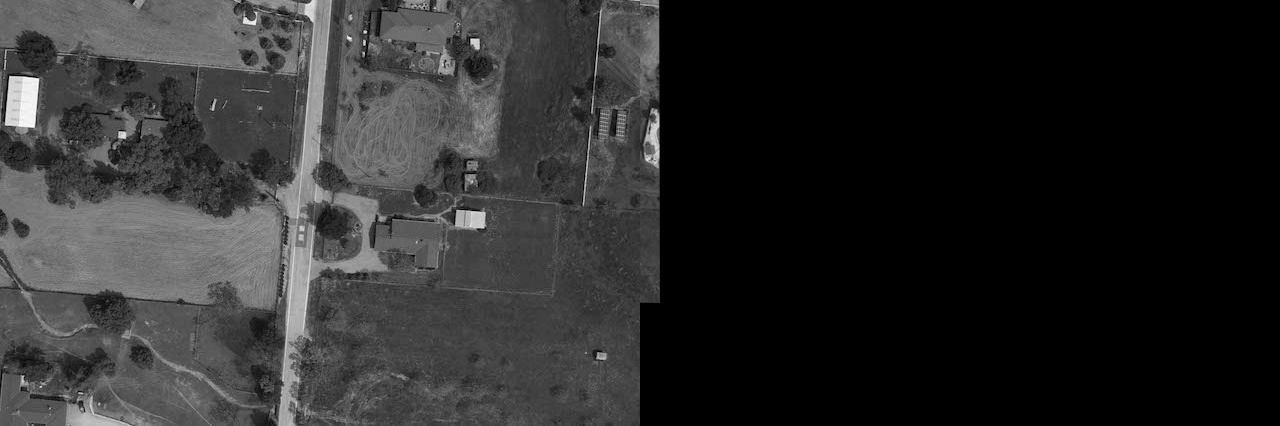
\includegraphics[width=7cm]{figures/brief_persp_foto2.jpeg}
\caption{brief\_persp\_foto2.jpeg} \label{brief_persp_foto2}
\end{center}
\end{figure}

\begin{figure}[H]
\begin{center}
	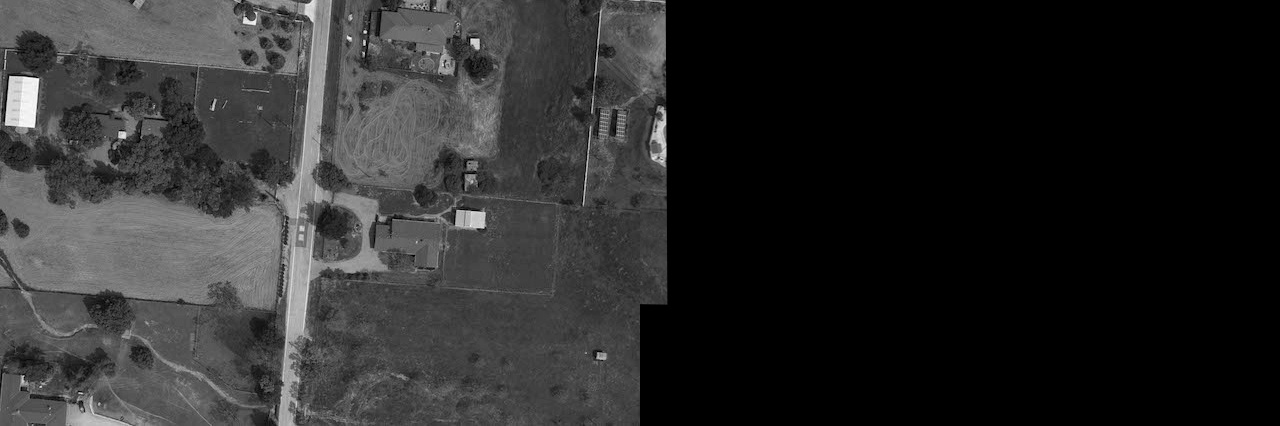
\includegraphics[width=7cm]{figures/orb_persp_foto2.jpeg}
\caption{orb\_persp\_foto2.jpeg} \label{orb_persp_foto2}
\end{center}
\end{figure}

\begin{figure}[H]
\begin{center}
	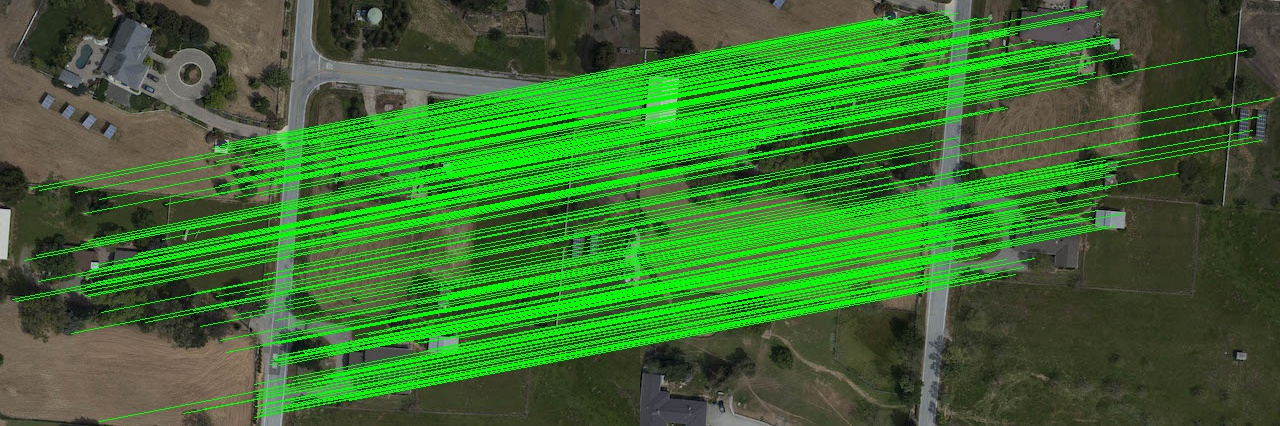
\includegraphics[width=7cm]{figures/sift_vis_foto2.jpeg}
\caption{sift\_vis\_foto2.jpeg} \label{sift_vis_foto2}
\end{center}
\end{figure}

\begin{figure}[H]
\begin{center}
	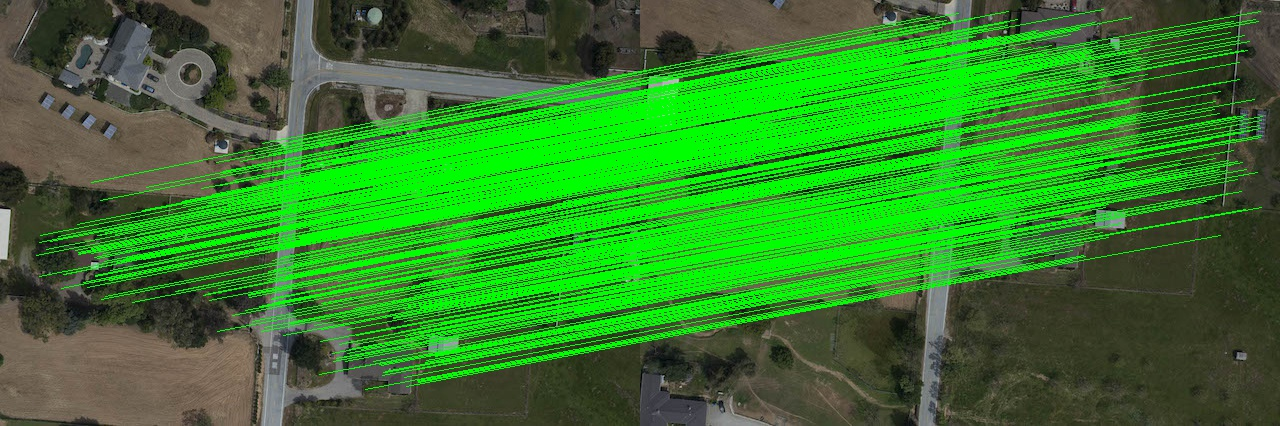
\includegraphics[width=7cm]{figures/surf_vis_foto2.jpeg}
\caption{surf\_vis\_foto2.jpeg} \label{surf_vis_foto2}
\end{center}
\end{figure}

\begin{figure}[H]
\begin{center}
	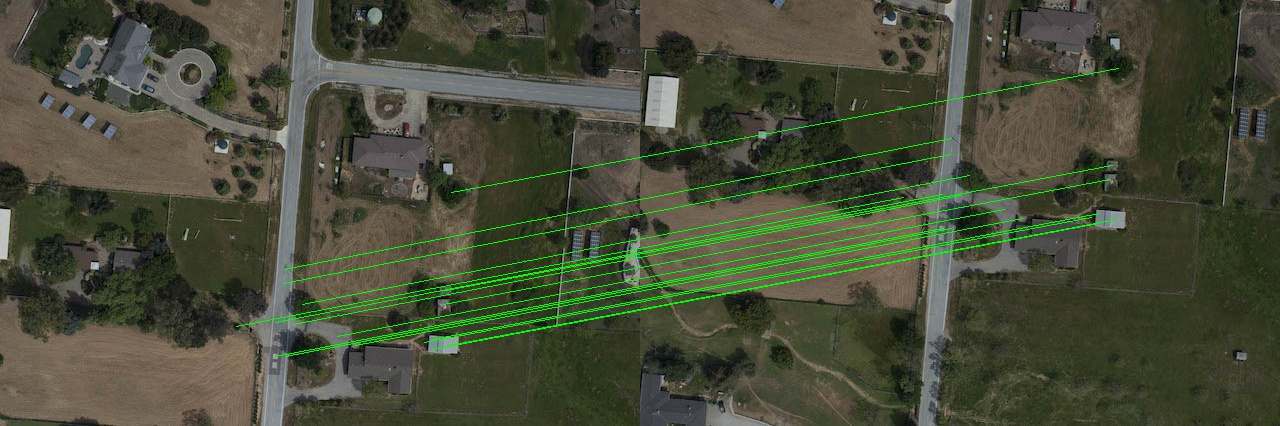
\includegraphics[width=7cm]{figures/brief_vis_foto2.jpeg}
\caption{brief\_vis\_foto2.jpeg} \label{brief_vis_foto2}
\end{center}
\end{figure}

\begin{figure}[H]
\begin{center}
	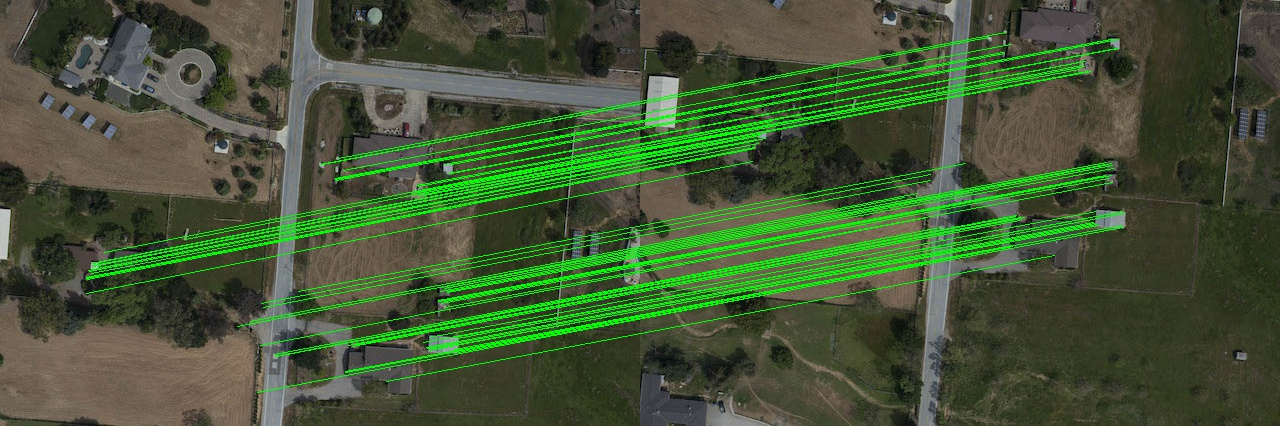
\includegraphics[width=7cm]{figures/orb_vis_foto2.jpeg}
\caption{orb\_vis\_foto2.jpeg} \label{orb_vis_foto2}
\end{center}
\end{figure}

\end{document}
